\subsection{Sensitivity of the primary independently calibrated study}\label{app:calibrated-sensitivity-v83}
This post hoc analysis uses the saved endpoints from the primary independently calibrated twelve-condition experiment, with its same fixed candidates, reference statistics, row pools and completed-evidence clocks. It reclassifies all twelve conditions over $[0,1]\,\mathrm{K}^2$ at five/ten seconds; every original endpoint and its adjacent floating values enter the grid. The primary tolerance remains $0.25\,\mathrm{K}^2$. At ten seconds the counts are 10 STOP/1 violation/1 unresolved for each reduced proposal, 9/1/2 for full search and 9/0/3 for the common coarse bound.

For the additional pool-79011 concentrated STOP, all three reduced methods satisfy STOP while full search remains unresolved on
\[
 \tau\in[0.24194363619769974,\,0.3083408101900695)\,\mathrm{K}^2.
\]
The closed decimal interval $[0.242,0.308]\,\mathrm{K}^2$ is conservative. The corresponding common-advantage interval is empty at five seconds.

\begin{figure*}[t]\centering
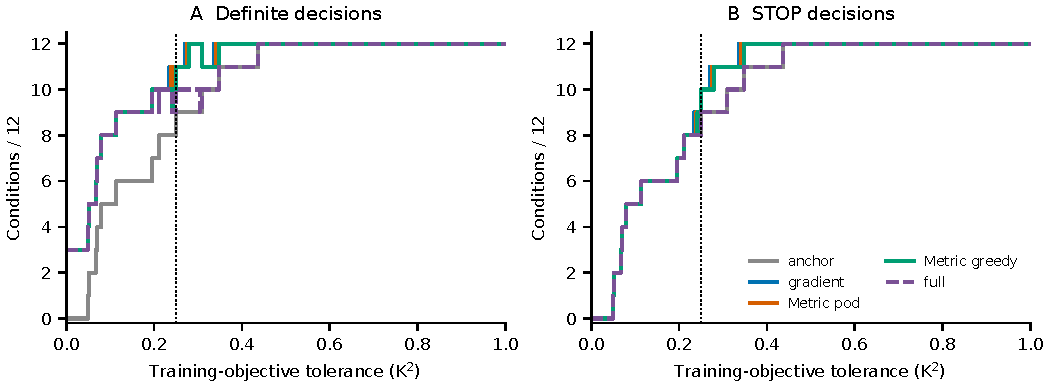
\includegraphics[width=\textwidth]{images/calibration_threshold_v83.pdf}
\caption{Threshold sensitivity for the primary independently calibrated twelve-condition study, using each method's own evidence completed by ten seconds. The vertical line is the unchanged $0.25\,\mathrm{K}^2$ primary tolerance. Curves reclassify the saved primary-threshold runs; early coarse STOPs can have skipped search. They do not represent a rerun of the acquisition policy at every new tolerance.}\label{fig:calibrated-sensitivity-v83}
\end{figure*}

Scalar endpoint manifests regenerate these curves without solver execution. 
